\subsection{Backend Tests}
The backend is a key part of the system as it handles all business logic and data storage in the system. Because 
the DBAccess class was made as a facade it made the most sense to us to do blackbox testing of it, as users of
the class would not have knowledge of its internal logic. The tests are done as automated unit tests to allow them
to be run everytime changes are made in backend part of the system, thereby ensuring that everything is working as
intended.

To try to maximise the coverage in our backend tests we made a coverage table (see figure \ref{fig:covtabs} for an example,
or appendix \ref{app:covtabs}) which describes what inputs tests should be made for. Having the coverage table at hand
when implementing the tests was great as it ensured that we had the wanted coverage for all methods. It also allowed us
 to split the implementation of the tests between us but still have the same coverage level as the coverage table was done
 in collaboration.

\begin{figure}[hbt]
	\centering
	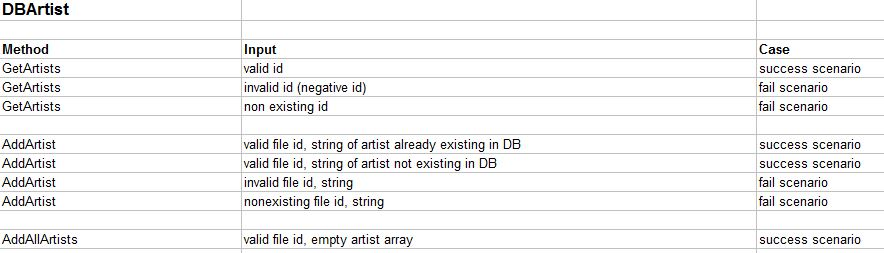
\includegraphics[scale=0.52]{./testing/coverage.jpg}
	\caption{Part of the coverage table for the backend tests}
	\label{fig:covtabs}
\end{figure}
  
